\documentclass[compress]{beamer}
\usecolortheme{default}

\usepackage{lmodern, epstopdf, multirow, array, setspace, bbm, tcolorbox, pbox, bm, mathtools, tikz}
\usepackage[T1]{fontenc}

\setbeamertemplate{frametitle}[default][center]
\setbeamertemplate{footline}{\hfill \insertframenumber/\inserttotalframenumber\hspace*{5pt}\vspace{5pt}}
\setbeamertemplate{navigation symbols}{}

\newlength{\wideitemsep}
\setlength{\wideitemsep}{\itemsep}
\addtolength{\wideitemsep}{4pt}
\let\olditem\item
\renewcommand{\item}{\setlength{\itemsep}{\wideitemsep}\olditem}
\setlength{\leftmargini}{12pt}
\setlength{\leftmarginii}{14pt}
\setbeamertemplate{itemize/enumerate subbody begin}{\vspace{6pt}}
\setbeamertemplate{itemize item}[circle]
\setbeamertemplate{enumerate item}[circle]
\setbeamertemplate{enumerate subitem}[default]

\setbeamercolor{alerted text}{fg=blue}
\setbeamersize{text margin left=1.5em,text margin right=1.5em}

\tcbset{
    colback=white,
    colframe=black,
    coltext=black,
    coltitle=blue,
    colbacktitle=white,
    boxrule=1pt,
    titlerule=0pt,
    toptitle=4pt,
    top=2pt
}

\newenvironment{changemargin}[2]{% 
  \begin{list}{}{% 
    \setlength{\topsep}{0pt}% 
    \setlength{\leftmargin}{#1}% 
    \setlength{\rightmargin}{#2}% 
    \setlength{\listparindent}{\parindent}% 
    \setlength{\itemindent}{\parindent}% 
    \setlength{\parsep}{\parskip}% 
  }% 
  \item[]}{\end{list}}
  
\newenvironment{defn}{%
  \begin{tcolorbox}[title={Definition}]%
  }{\end{tcolorbox}}
  
\newenvironment{prop}[1]{%
  \begin{tcolorbox}[title={Proposition #1}]%
  }{\end{tcolorbox}}
  
\newcommand{\cit}[1]{{\footnotesize \textcolor[rgb]{0.5,0,0}{#1}}}

% Font size for code listings (verbatim blocks); reset with \normalsize
\newcommand{\codesize}{\fontsize{7}{8.5}\selectfont}

\newcommand{\slidesetup}[1]{%
  \title{#1}%
  \subtitle{\texorpdfstring{\vspace{0.3\baselineskip}}{} {\small This version: \today}}%
  \author[Mikkel Plagborg-Moller]{ECMA 31150, Spring 2026 \texorpdfstring{\\[0.5ex]}{} University of Chicago \texorpdfstring{\\[0.5ex]}{} Department of Economics \texorpdfstring{\\[4ex]}{} Mikkel Plagborg-Moller}%
  \date{}%
}

% \circleoverlay[options]{text}
% Draws a red circle with a text box nearby on a tikz overlay.
% Options (with defaults):
%   cx=0cm, cy=0cm      - circle center (shift from page center)
%   r=1cm               - circle radius
%   tx=0cm, ty=0cm      - text box offset from circle center
%   text anchor=east    - anchor of text node (east = text left, west = text right)
%   font=\normalsize    - font size for text
\pgfkeys{
  /circleoverlay/.cd,
  cx/.store in=\cocx, cx=0cm,
  cy/.store in=\cocy, cy=0cm,
  r/.store in=\cor, r=1cm,
  tx/.store in=\cotx, tx=0cm,
  ty/.store in=\coty, ty=0cm,
  text anchor/.store in=\cotextanchor, text anchor=east,
  font/.store in=\cofont, font=\normalsize,
}
\newcommand{\circleoverlay}[2][]{%
  \pgfkeys{/circleoverlay/.cd, cx=0cm, cy=0cm, r=1cm, tx=0cm, ty=0cm, text anchor=east, font=\normalsize, #1}%
  \pgfmathsetlengthmacro{\circlediameter}{2*\cor}%
  \node[draw=red, line width=2pt, circle, minimum size=\circlediameter, inner sep=0pt]
    (tmpcirc) at ([xshift=\cocx,yshift=\cocy]current page.center) {};%
  \node[anchor=\cotextanchor, fill=white, draw=red, text=red, inner sep=4pt, align=left, font=\cofont]
    at ([xshift=\cotx,yshift=\coty]tmpcirc.center) {#2};%
}

\DeclareMathOperator*{\argmax}{argmax}
\DeclareMathOperator*{\argmin}{argmin}
\DeclareMathOperator{\diag}{diag}
\DeclareMathOperator{\var}{Var}
\DeclareMathOperator{\cov}{Cov}
\DeclareMathOperator{\corr}{Corr}
\DeclareMathOperator{\lrv}{LRV}


\slidesetup{Vector autoregression I}

\begin{document}
\frame{
\maketitle
}

\frame{
\frametitle{Plan for this slide deck}
\begin{enumerate}
\item Analysis of multiple time series
\begin{itemize}
\item Cross-correlogram
\end{itemize}
\item Autoregressive distributed lag model
\item Granger causality: which variables predict each other?
\item Vector autoregression
\end{enumerate}
}

\frame{
\frametitle{Multiple time series}
\begin{itemize}
\item So far we've discussed how to model a single time series $\lbrace y_t \rbrace$.
\item But in practice we have access to 1000s of macro time series.
\begin{itemize}
\item There are more than 800k on FRED, and counting!
\end{itemize}
\item We often want to study the relationship between two or more series.
\item We want to forecast using several relevant predictors.
\end{itemize}
}

\frame{
\frametitle{Cross-correlogram}
\begin{itemize}
\item Take two (jointly) covariance stationary time series, $y_t$ and $x_t$.
\item Define the population \textbf{cross-correlogram}:
\[\rho_{y,x}(\ell) \equiv \corr(y_t,x_{t-\ell}).\]
Measures how much lags (or leads) of $x$ predict $y$.
\begin{itemize}
\item \alert{Exercise:} show that $\rho_{y,x}(-\ell) = \rho_{x,y}(\ell)$.
\end{itemize}
\item Natural estimator is the sample cross-correlogram:
\[\hat{\rho}_{y,x}(\ell) \equiv \begin{cases}
\frac{1}{T}\sum_{t=\ell+1}^T (y_t-\bar{y})(x_{t-\ell}-\bar{x})/(\hat{\sigma}_y\hat{\sigma}_x) & \text{for } \ell \geq 0, \\
\hat{\rho}_{x,y}(-\ell) & \text{for } \ell<0,
\end{cases}\]
where $\hat{\sigma}_y,\hat{\sigma}_x$ are the sample standard deviations.
\end{itemize}
}

\frame{
\begin{figure}
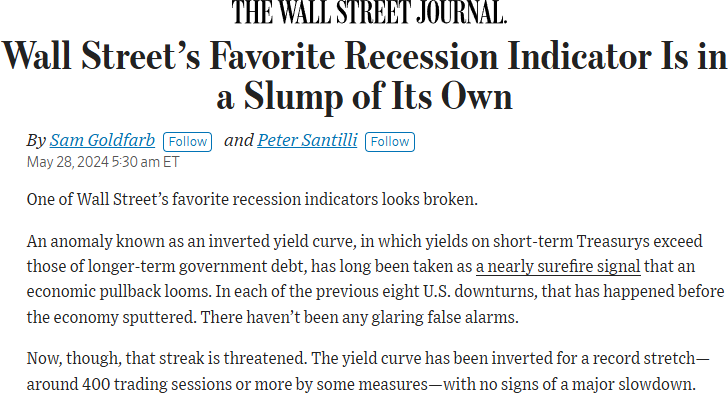
\includegraphics[width=\linewidth]{fig/wsj_inversion.png} \\
\bigskip
\scriptsize \url{https://www.wsj.com/finance/investing/wall-streets-favorite-recession-indicator-is-in-a-slump-of-its-own-ee885cb9}
\end{figure}
}

\frame{
\begin{figure}
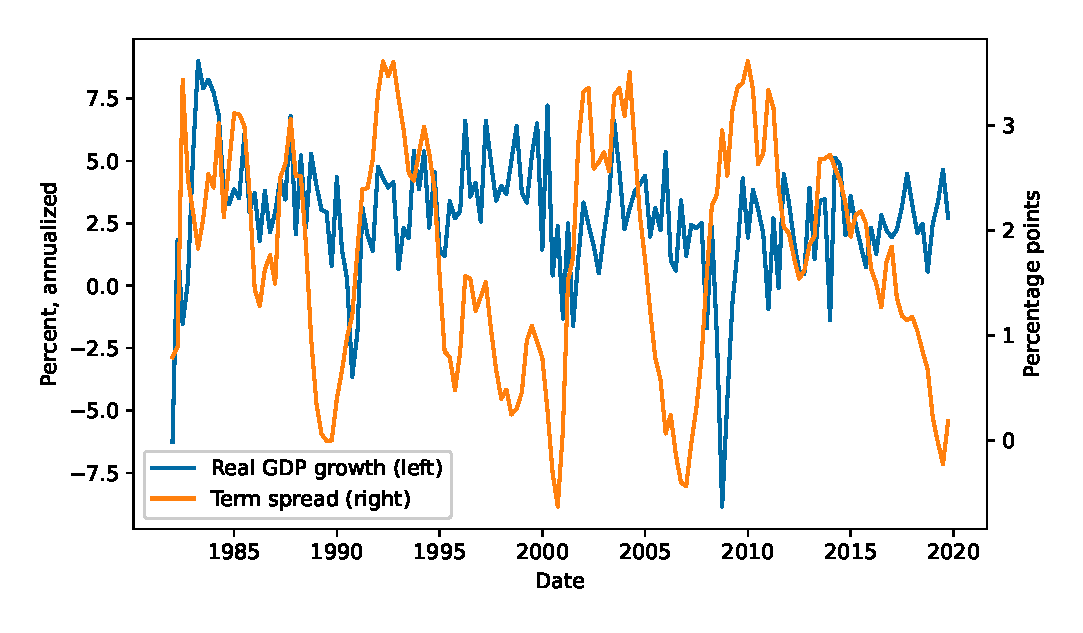
\includegraphics[width=\linewidth]{fig/gdp_spread.eps} \\
Term spread = difference between yields on 10-year and 3-month U.S.\ Treasury bonds
\end{figure}
}

\frame{
\begin{figure}
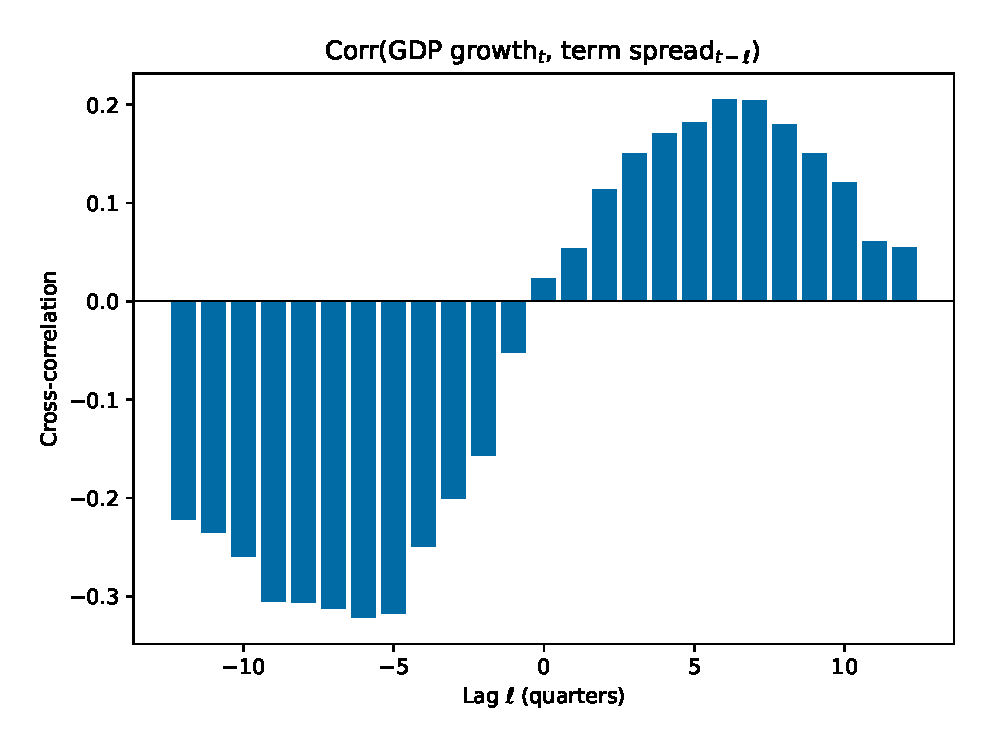
\includegraphics[width=\linewidth]{fig/correlogram.eps}
\end{figure}
}

\frame{
\frametitle{Autoregressive distributed lag model}
\begin{itemize}
\item To use $\lbrace x_t \rbrace$ for forecasting $\lbrace y_t \rbrace$, we can add its lags as additional covariates in an AR specification:
\[y_t = c + a_1y_{t-1} + \dots + a_p y_{t-p} + b_1 x_{t-1} + \dots + b_q x_{t-q} + u_t,\]
where we assume
\[E[u_t \mid \lbrace y_s,x_s \rbrace_{s<t}] = 0.\]
\item Called an \textbf{autoregressive distributed lag} (ADL) model.
\item Optimal forecast:
\begin{align*}
y_{t|t-1} &\equiv E[y_t \mid \lbrace y_s,x_s \rbrace_{s<t}] \\
&= c + a_1y_{t-1} + \dots + a_p y_{t-p} + b_1 x_{t-1} + \dots + b_q x_{t-q}.
\end{align*}
\item Estimate parameters by OLS w.\ heteroskedasticity-robust SE.
\end{itemize}
}

\begin{frame}[fragile]
\footnotesize
\begin{verbatim}
n_lags = 2

# Generate lagged variables
reg_df = df[['growth', 'spread']].copy()
for l in range(1, n_lags + 1):
    reg_df[f'growth_lag{l}'] = reg_df['growth'].shift(l)
    reg_df[f'spread_lag{l}'] = reg_df['spread'].shift(l)

# OLS estimation
y = reg_df['growth']
X_cols = [f'growth_lag{l}' for l in range(1, n_lags + 1)] + \
    [f'spread_lag{l}' for l in range(1, n_lags + 1)]
         
X = sm.add_constant(reg_df[X_cols])

model = sm.OLS(y, X, missing='drop').fit(cov_type='HC1')
print(model.summary())
\end{verbatim}
\end{frame}

\begin{frame}[fragile]
\scriptsize
\begin{verbatim}
                            OLS Regression Results                            
==============================================================================
Dep. Variable:                 growth   R-squared:                       0.260
Model:                            OLS   Adj. R-squared:                  0.239
Method:                 Least Squares   F-statistic:                     11.49
Date:                Mon, 06 Apr 2026   Prob (F-statistic):           3.94e-08
Time:                        09:28:26   Log-Likelihood:                -322.65
No. Observations:                 150   AIC:                             655.3
Df Residuals:                     145   BIC:                             670.4
Df Model:                           4                                         
Covariance Type:                  HC1                                         
===============================================================================
                  coef    std err          z      P>|z|      [0.025      0.975]
-------------------------------------------------------------------------------
const           0.9231      0.409      2.259      0.024       0.122       1.724
growth_lag1     0.3438      0.105      3.280      0.001       0.138       0.549
growth_lag2     0.2128      0.080      2.652      0.008       0.056       0.370
spread_lag1    -0.2585      0.304     -0.849      0.396      -0.855       0.338
spread_lag2     0.4460      0.329      1.355      0.175      -0.199       1.091
==============================================================================
\end{verbatim}
\begin{center}
\normalsize (rest of output omitted)
\end{center}
\end{frame}

\begin{frame}
\frametitle{Granger causality}
\begin{itemize}
\item We say that $\lbrace x_t \rbrace$ \textbf{Granger-causes} $\lbrace y_t \rbrace$ if the former provides any additional forecasting power over and above lags of the latter:
\[E[y_t \mid \lbrace y_s,x_s \rbrace_{s<t}] \neq E[y_t \mid \lbrace y_s \rbrace_{s<t}].\]
\vspace{-1.5\baselineskip}
\begin{itemize}
\item Confusing terminology: this is not about causal inference in the counterfactual (\emph{ceteris paribus}) sense.
\item ``The weather forecast Granger-causes the weather.''
\end{itemize}
\item In the ADL model
\[y_t = c + a_1y_{t-1} + \dots + a_p y_{t-p} + b_1 x_{t-1} + \dots + b_q x_{t-q} + u_t,\]
$\lbrace x_t \rbrace$ Granger-causes $\lbrace y_t \rbrace$ if and only if $b_\ell \neq 0$ for at least one $\ell=1,\dots,q$.
\begin{itemize}
\item Use F-test to test null hypothesis of no Granger causality.
\end{itemize}
\end{itemize}
\end{frame}

\begin{frame}[fragile]
\scriptsize
\begin{verbatim}
spread_lags = [f'spread_lag{l}' for l in range(1, n_lags + 1)]
restriction = ' = '.join(spread_lags) + ' = 0'
f_test = model.f_test(restriction)
print(restriction)
print(f_test)
\end{verbatim}
\medskip
\normalsize
\textbf{Result:}
\scriptsize
\begin{verbatim}
spread_lag1 = spread_lag2 = 0
<F test: F=1.2094836277525283, p=0.30134309292175676, df_denom=145, df_num=2>
\end{verbatim}
\medskip
\normalsize
Can't reject that the spread does \emph{not} Granger-cause growth.
\end{frame}

\frame{
\begin{figure}
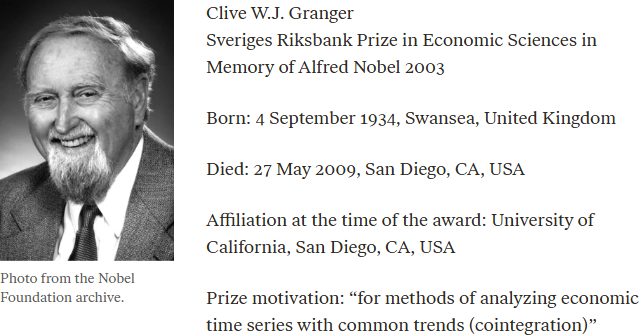
\includegraphics[width=0.8\linewidth]{fig/granger.png} \\
\bigskip
\scriptsize
\url{https://www.nobelprize.org/prizes/economic-sciences/2003/granger/facts/}
\end{figure}
}

\frame{
\frametitle{ADL model: multi-step forecast}
\begin{itemize}
\item Consider ADL model with $p=q=1$:
\[y_t = c + \rho y_{t-1} + b x_{t-1} + u_t.\]
\item How to forecast two periods ahead?
\begin{align*}
y_{t+2} &= c + \rho y_{t+1} + b x_{t+1} + u_{t+2} \\
&= c + \rho (c + \rho y_t + b x_t + u_{t+1}) + b x_{t+1} + u_{t+2}
\end{align*}
\[\Downarrow\]
\[E[y_{t+2} \mid \lbrace y_s,x_s\rbrace_{s \leq t}] = (1+\rho)c + \rho^2y_t + \rho b x_t + b E[x_{t+1} \mid \lbrace y_s,x_s\rbrace_{s \leq t}].\]
\item But the model doesn't tell us what the last conditional expectation equals. \\
$\Longrightarrow$ Solution: specify a second ADL model for $x_t$!
\end{itemize}
}

\frame{
\frametitle{Vector autoregression}
\begin{itemize}
\item ADL models for both $y_t$ and $x_t$ (new notation):
\begin{align*}
y_t &= c_1 + A_{11}y_{t-1} + A_{12} x_{t-1} + u_{1t},\\
x_t &= c_2 + A_{21}y_{t-1} + A_{22} x_{t-1} + u_{2t},
\end{align*}
\[E[u_{jt} \mid \lbrace y_s,x_s \rbrace_{s<t}] = 0,\quad j=1,2.\]
\item Convenient to write this with vectors and matrices:
\[\bm{y}_t = \bm{c} + \bm{A}\bm{y}_{t-1} + \bm{u}_t,\quad E[\bm{u}_t \mid \lbrace \bm{y}_s \rbrace_{s<t}]=\bm{0},\quad \text{where}\]
\[\bm{y}_t \equiv \begin{pmatrix}
y_t \\
x_t
\end{pmatrix},\quad \bm{c} \equiv \begin{pmatrix}
c_1 \\
c_2
\end{pmatrix},\quad \bm{A} \equiv \begin{pmatrix}
A_{11} & A_{12} \\
A_{21} & A_{22}
\end{pmatrix},\quad \bm{u}_t \equiv \begin{pmatrix}
u_{1t} \\
u_{2t}
\end{pmatrix}.\]
\item Called a \textbf{vector autoregression} of lag order 1, VAR(1).
\end{itemize}
}

\frame{
\begin{figure}
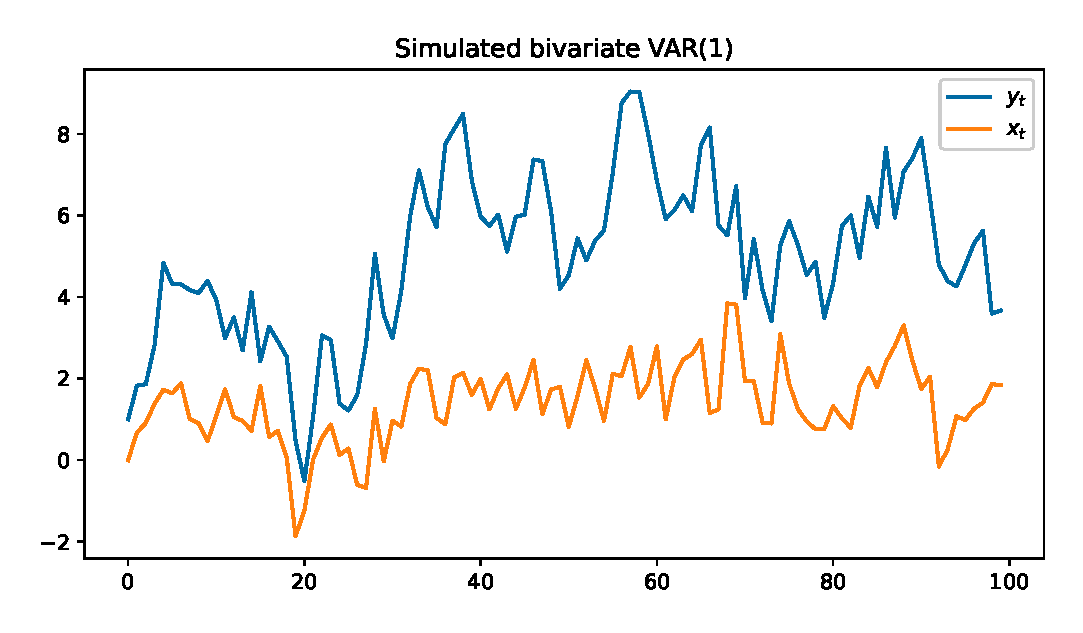
\includegraphics[width=\linewidth]{fig/var_sim.eps} \\
\[\bm{y}_t = \begin{pmatrix}
1 \\
0
\end{pmatrix} + \begin{pmatrix}
0.8 & 0.1 \\
0.2 & 0.3
\end{pmatrix} \bm{y}_{t-1} + \bm{u}_t,\quad \bm{u}_t \overset{iid}{\sim} N\left(\bm{0},\begin{pmatrix}
1 & 0.3 \\
0.3 & 0.5
\end{pmatrix}\right)\]
\end{figure}
}

\frame{
\frametitle{VAR(1): more variables}
\begin{itemize}
\item With the vector notation, we can easily generalize our model to contain $n$ variables:
\[\bm{y}_t = \bm{c} + \bm{A}\bm{y}_{t-1} + \bm{u}_t,\quad E[\bm{u}_t \mid \lbrace \bm{y}_s \rbrace_{s<t}]=\bm{0},\quad \text{where}\]
\[\bm{y}_t \equiv \underbrace{\begin{pmatrix}
y_{1t} \\
\vdots \\
y_{nt}
\end{pmatrix}}_{n \times 1},\quad \bm{c} \equiv \underbrace{\begin{pmatrix}
c_1 \\
\vdots \\
c_n
\end{pmatrix}}_{n \times 1},\quad \bm{A} \equiv \underbrace{\begin{pmatrix}
A_{11} & \cdots & A_{1n} \\
\vdots & \ddots & \vdots \\
A_{n1} & \cdots & A_{nn}
\end{pmatrix}}_{n \times n},\quad \bm{u}_t \equiv \underbrace{\begin{pmatrix}
u_{1t} \\
\vdots \\
u_{nt}
\end{pmatrix}}_{n \times 1}.\]
\item Henceforth I will be using the $y_{it}$ notation, not $y_t$ and $x_t$.
\end{itemize}
}

\frame{
\frametitle{VAR(1): innovations}
\begin{itemize}
\item The innovation process $\lbrace \bm{u}_t \rbrace$ is \textbf{multivariate white noise}:
\[\corr(u_{it},u_{j,t-\ell}) = 0\quad \text{for all } \ell \neq 0 \text{ and } i,j \in \lbrace 1,\dots,n \rbrace,\]
i.e., the cross-correlogram between $\lbrace u_{it} \rbrace$ and $\lbrace u_{jt} \rbrace$ is 0 at all leads and lags $\ell \neq 0$.
\item We still allow the elements of $\bm{u}_t$ to be \emph{contemporaneously} correlated:
\[\bm{\Sigma} \equiv \var(\bm{u}_t) = \begin{pmatrix}
\var(u_{1t}) & \cov(u_{1t},u_{2t}) & \cdots & \cov(u_{1t},u_{nt}) \\
\cov(u_{2t},u_{1t}) & \var(u_{2t}) & \cdots & \cov(u_{2t},u_{nt}) \\
\vdots & & \ddots & \vdots \\
\cov(u_{nt},u_{1t}) & \cov(u_{nt},u_{2t}) & \cdots & \var(u_{nt})
\end{pmatrix}\]
need not be a diagonal matrix.
\end{itemize}
}

\frame{
\frametitle{VAR(1): moments}
\[\bm{y}_t = \bm{c} + \bm{A}\bm{y}_{t-1} + \bm{u}_t\]
\vspace{-0.5\baselineskip}
\begin{itemize}
\item Suppose $\lbrace \bm{y}_t \rbrace$ is covariance stationary. Then
\[E[\bm{y}_t] = \bm{c} + \bm{A} E[\bm{y}_t] \quad \Longrightarrow \quad \boxed{E[\bm{y}_t] = (\bm{I}-\bm{A})^{-1}\bm{c}},\]
where $\bm{I}$ is the $n \times n$ identity matrix.
\item Moreover, we can solve for $\var(\bm{y}_t)$ through the ``Lyapunov equations''
\[\boxed{\var(\bm{y}_t) = \bm{A}\var(\bm{y}_t) \bm{A}' + \bm{\Sigma}}.\]
\item Finally,
\begin{align*}
\cov(\bm{y}_t,\bm{y}_{t-\ell}) &= \bm{A}\cov(\bm{y}_{t-1},\bm{y}_{t-\ell}) = \bm{A}^2\cov(\bm{y}_{t-2},\bm{y}_{t-\ell}) \\
&= \dots = \boxed{\bm{A}^\ell \var(\bm{y}_t)}.
\end{align*}
\end{itemize}
}

\frame{
\frametitle{VAR(1): forecasting}
\begin{itemize}
\item One-step-ahead forecast:
\[\bm{y}_{t+1|t} \equiv E[\bm{y}_{t+1} \mid \lbrace \bm{y}_s \rbrace_{s\leq t}] = E[\bm{y}_{t+1} \mid \bm{y}_t] = \boxed{\bm{c} + \bm{A}\bm{y}_t}.\]
\item Multi-step forecast:
\begin{align*}
\bm{y}_{t+h|t} &\equiv E[\bm{y}_{t+h} \mid \lbrace \bm{y}_s \rbrace_{s\leq t}] = E[\bm{y}_{t+h} \mid \bm{y}_t] \\
&= \sum_{j=0}^{h-1} \bm{A}^j\bm{c} + \bm{A}^h\bm{y}_t = \boxed{(\bm{I}-\bm{A})^{-1}(\bm{I}-\bm{A}^h)\bm{c} + \bm{A}^h\bm{y}_t}.
\end{align*}
\item \alert{Exercise:} verify these.
\end{itemize}
}

\frame{
\frametitle{VAR(1): estimation}
\begin{itemize}
\item Since a VAR is just a system of ADL models, we can estimate them in the same way: run an OLS regression \emph{separately} for each of the $n$ equations in the system.
\[y_{it} = \hat{c}_i + \hat{A}_{i1}y_{1,t-1} + \dots + \hat{A}_{in}y_{n,t-1} + \hat{u}_{it},\quad i=1,\dots,n.\]
\item Then stack to get estimators of the parameter vectors/matrices:
\[\hat{\bm{c}} \equiv \begin{pmatrix}
\hat{c}_1 \\
\vdots \\
\hat{c}_n
\end{pmatrix},\quad \hat{\bm{A}} \equiv \begin{pmatrix}
\hat{A}_{11} & \cdots & \hat{A}_{1n} \\
\vdots & \ddots & \vdots \\
\hat{A}_{n1} & \cdots & \hat{A}_{nn}
\end{pmatrix},\quad \hat{\bm{u}}_t \equiv \begin{pmatrix}
\hat{u}_{1t} \\
\vdots \\
\hat{u}_{nt}
\end{pmatrix},\]
\[\hat{\bm{\Sigma}} \equiv \frac{1}{T-1} \sum_{t=2}^T \hat{\bm{u}}_t \hat{\bm{u}}_t'.\]
\end{itemize}
}

\frame{
\frametitle{VAR(1): properties of OLS estimator}
\begin{itemize}
\item One can prove that under similar conditions to AR($p$) models (including stationarity), the VAR OLS estimator is\dots
\begin{enumerate}
\item Consistent.
\item Biased in finite samples.
\item Asymptotically normal. Standard errors can be computed \emph{as if} we were running OLS regressions on i.i.d.\ data.
\end{enumerate}
\end{itemize}
}

\frame{
\frametitle{VAR(1): stationarity}
\begin{equation} \label{eqn:var}
\bm{y}_t = \bm{c} + \bm{A}\bm{y}_{t-1} + \bm{u}_t \tag{$\dagger$}
\end{equation}
\begin{itemize}
\item When is the VAR(1) model covariance stationary?
\item Suppose the square matrix $\bm{A}$ is diagonalizable:
\[\bm{A} = \bm{V}\bm{\Lambda}\bm{V}^{-1},\quad \bm{\Lambda}=\diag(\lambda_1,\dots,\lambda_n).\]
Here $\lambda_1,\dots,\lambda_n$ are the eigenvalues and the columns of $\bm{V}$ are the corresponding eigenvectors. Assume these are real for now.
\item Insert into the VAR equation (\ref{eqn:var}) and pre-multiply by $\bm{V}^{-1}$ to get
\[\bm{y}_t^* = \bm{c}^* + \bm{\Lambda}\bm{y}_{t-1}^* + \bm{u}_t^*,\quad \text{where}\]
\[\bm{y}_t^* \equiv \bm{V}^{-1}\bm{y}_t,\quad \bm{c}^* \equiv \bm{V}^{-1}\bm{c},\quad \bm{u}_t^* \equiv \bm{V}^{-1}\bm{u}_t.\]
\end{itemize}
}

\frame{
\frametitle{VAR(1): stationarity (cont.)}
\[\bm{y}_t^* = \bm{c}^* + \bm{\Lambda}\bm{y}_{t-1}^* + \bm{u}_t^*,\quad \text{where}\quad \bm{y}_t^* \equiv \bm{V}^{-1}\bm{y}_t\]
\vspace{-0.5\baselineskip}
\begin{itemize}
\item Recall $\bm{\Lambda}=\diag(\lambda_1,\dots,\lambda_n)$. Hence, if we write each of the above $n$ equations out explicitly, we get
\[y_{it}^* = c_i^* + \lambda_i y_{i,t-1}^* + u_{it}^*,\quad i=1,\dots,n.\]
So each of the $n$ series $y_{it}^*$ follows a univariate AR(1) process!
\item These univariate processes are cov.\ stationary if and only if $|\lambda_i| < 1$ for all $i$.
\item Clearly, $\bm{y}_t = \bm{V}\bm{y}_t^*$ is cov.\ stationary if and only if $\bm{y}_t^*$ is.
\item \alert{Result:} The original VAR(1) model for $\bm{y}_t$ has a cov.\ stationary solution if and only if all eigenvalues of $\bm{A}$ satisfy $|\lambda_i| < 1$.
\end{itemize}
}

\frame{
\frametitle{VAR(1): stationarity (cont.)}
\begin{itemize}
\item Turns out the previous proof can be extended to the case where $\bm{A}$ is not diagonalizable, using the ``Jordan decomposition''.
\item Moreover, if some eigenvalues of $\bm{A}$ are complex numbers, the condition for cov.\ stationarity remains $|\lambda_i| < 1$.
\begin{itemize}
\item That is, all $n$ eigenvalues must be strictly \emph{inside} the unit circle in the complex plane.
\item Recall: the absolute value of a complex number is sometimes called the \textbf{modulus}.
\end{itemize}
\end{itemize}
}

\frame{
\frametitle{VAR($p$) model}
\begin{itemize}
\item \textbf{VAR($p$) model}:
\[\bm{y}_t = \bm{c} + \bm{A}_1\bm{y}_{t-1} + \dots + \bm{A}_p\bm{y}_{t-p} + \bm{u}_t,\quad E[\bm{u}_t \mid \lbrace \bm{y}_s \rbrace_{s<t}]=\bm{0}.\]
\item Write out equation $i$ explicitly:
\[y_{it} = c_i + \sum_{\ell=1}^p \sum_{j=1}^n A_{\ell,ij} y_{j,t-\ell} + u_{it},\]
where $A_{\ell,ij}$ is the $(i,j)$ element of $\bm{A}_\ell$.
\item Each variable $i$ depends on $p$ lags of all $n$ variables $y_{jt}$, $j=1,\dots,n$.
\item Estimation: separate OLS regression in each of the $n$ equations.
\begin{itemize}
\item Number of covariates in each equation: $n \times p$ (plus one intercept).
\end{itemize}
\end{itemize}
}

\frame{
\frametitle{VAR: lag order selection}
\begin{itemize}
\item Could do general-to-specific testing.
\item Information criteria:
\begin{align*}
\mathit{BIC}(p) &\equiv \log\left(\det\left(\hat{\bm{\Sigma}}(p)\right)\right) + n(1+np)\frac{\log T_\text{eff}}{T_\text{eff}}, \\
\mathit{AIC}(p) &\equiv \log\left(\det\left(\hat{\bm{\Sigma}}(p)\right)\right) + n(1+np)\frac{2}{T_\text{eff}},
\end{align*}
where $\det(\hat{\bm{\Sigma}}(p))$ is the determinant of $\hat{\bm{\Sigma}}(p)$ (the residual var-cov matrix from a VAR regression with $p$ lags).
\item Note: a VAR has $n$ equations, each with $1+np$ coefficients.
\end{itemize}
}

\frame{
\frametitle{Practical coding}
\begin{itemize}
\item In practice, we don't explicitly run $n$ separate OLS regressions.
\item Instead, most statistics programming languages have built-in VAR estimation routines.
\item Python: {\tt statsmodels.tsa.VAR}.
\begin{itemize}
\item Can also do lag order selection.
\item Caveat: standard errors computed under the assumption of i.i.d.\ (and thus homoskedastic) shocks. This is conventional in the literature.
\end{itemize}
\end{itemize}
}

\begin{frame}[fragile]
\begin{verbatim}
# Lag order selection
var_model = sm.tsa.VAR(df[['growth', 'spread']])
lag_order = var_model.select_order(maxlags=12)
print(lag_order.summary())

# Estimation
var_results = var_model.fit(ic='aic')
print(var_results.summary())
\end{verbatim}
\end{frame}

\begin{frame}[fragile]
\footnotesize
\begin{verbatim}
 VAR Order Selection (* highlights the minimums)  
==================================================
       AIC         BIC         FPE         HQIC   
--------------------------------------------------
0        1.850       1.892       6.362       1.867
1      -0.2777     -0.1517      0.7575     -0.2265
2     -0.5010*    -0.2909*     0.6060*    -0.4156*
3      -0.4799     -0.1857      0.6190     -0.3603
4      -0.4485    -0.07029      0.6388     -0.2948
5      -0.4239     0.03832      0.6549     -0.2361
6      -0.3939      0.1524      0.6751     -0.1719
7      -0.3414      0.2890      0.7120    -0.08523
8      -0.3104      0.4040      0.7350    -0.02005
9      -0.3407      0.4578      0.7137    -0.01623
10     -0.2924      0.5901      0.7499     0.06624
11     -0.3173      0.6493      0.7325     0.07549
12     -0.2991      0.7515      0.7472      0.1278
--------------------------------------------------
\end{verbatim}
\end{frame}

\begin{frame}[fragile]
\scriptsize
\begin{verbatim}
Results for equation growth
============================================================================
               coefficient       std. error           t-stat            prob
----------------------------------------------------------------------------
const             0.923150         0.408835            2.258           0.024
L1.growth         0.343830         0.079882            4.304           0.000
L1.spread        -0.258465         0.375531           -0.688           0.491
L2.growth         0.212839         0.077132            2.759           0.006
L2.spread         0.445969         0.378943            1.177           0.239
============================================================================

Results for equation spread
============================================================================
               coefficient       std. error           t-stat            prob
----------------------------------------------------------------------------
const             0.348306         0.085897            4.055           0.000
L1.growth        -0.010500         0.016783           -0.626           0.532
L1.spread         1.105984         0.078900           14.018           0.000
L2.growth        -0.039451         0.016206           -2.434           0.015
L2.spread        -0.225553         0.079617           -2.833           0.005
============================================================================
\end{verbatim}
\normalsize Note: growth equation coefficients same as earlier ADL regression.
\end{frame}

\begin{frame}[fragile]
\begin{verbatim}
Correlation matrix of residuals
            growth    spread
growth    1.000000  0.036940
spread    0.036940  1.000000
\end{verbatim}
\bigskip

Estimate of innovation var-cov matrix:
\[\hat{\bm{\Sigma}} \equiv \frac{1}{T-p}\sum_{t=p+1}^T \hat{\bm{u}}_t \hat{\bm{u}}_t',\]
where $\hat{\bm{u}}_t$ stacks the regression residuals from the $n$ OLS regressions, just like VAR(1) case.
\end{frame}

\frame{
\frametitle{What did we learn?}
\begin{itemize}
\item Cross-correlogram
\item ADL model, Granger causality
\item VAR(1) model
\begin{itemize}
\item Stationarity, moments
\item Forecasting
\item Estimation
\end{itemize}
\item VAR($p$) model
\begin{itemize}
\item Estimation
\item Lag length selection
\end{itemize}
\end{itemize}
}

\frame{
\frametitle{Looking ahead}
\begin{itemize}
\item In the VAR($p$) model, how do we\dots
\begin{itemize}
\item check stationarity?
\item forecast?
\item compute moments?
\end{itemize}
\item Multivariate VARMA model, matrix lag polynomials
\item VARs are biased in finite samples. How can we improve the accuracy of our VAR inference when the sample size is small?
\end{itemize}
}

\end{document}
